\documentclass[handout]{beamer}
\usepackage{pgfpages}\pgfpagesuselayout{4 on 1}[a4paper,landscape,border shrink=5mm]

\usepackage{xmpmulti,multimedia,xspace}
\usepackage[latin1]{inputenc}
\usepackage{tikz}
\usetikzlibrary{shadows}
\usepackage{anyfontsize}
\usepackage{graphicx}
\graphicspath{{./img/} }

%\usetheme{Berlin}
\usetheme{AnnArbor}

\setbeamercovered{invisible}
\setbeamersize{text margin left=7.5mm}
\setbeamersize{text margin right=7.5mm}

%==============================================================================

\begin{document}
\title{C Programming Tools: Part 1}
\subtitle{Building and Using your own Toolkit}
\institute[Imperial]{Dept of Computing, Imperial College London}
\date{21st May 2020}
\newcommand\RBox[1]{%
%  \tikz\node[draw,rounded corners,align=center,] {#1};%
  \tikz\node[draw,rounded corners,align=center,double copy shadow={opacity=0.3,shadow xshift=1ex,shadow yshift=-0.5ex,left color = brown!40,right color = magenta!80},left color=blue!50,right color=yellow!50 ] {#1};%
}  
\newcommand{\pitem}{\pause \item}
\setbeamerfont{author in head/foot}{size={\fontsize{3pt}{4pt}\selectfont}}
\author[Duncan White]
{%
   \texorpdfstring{
        \begin{columns}
            \column{.8\linewidth}
            \centering
            \RBox{Duncan C. White\\
            \href{mailto:d.white@imperial.ac.uk}{d.white@imperial.ac.uk}}
        \end{columns}
   }
   {Duncan C. White}
}

%\begin{frame}
%\titlepage
%\end{frame}

\begin{frame}[fragile]
\vspace*{.3cm}\titlepage  
\end{frame}

%\section*{Outline}
%\begin{frame}
%\tableofcontents
%\end{frame}

\section{Introduction}
\subsection{Toolkits and Craftsmanship}

\begin{frame}
\large
      \begin{itemize}
      \item
      As programmers, you will learn \alert{many languages} over your career.
      Right now, you're learning C - with Will Knottenbelt.
      \pause
      C is an excellent language to learn, long-lived (over 40 years old),
      still going strong, and \alert{irreplaceable in it's niches}.

      \pitem
      When learning a new language like C, there are \alert{several learning stages}
      before you achieve \alert{basic competence}:

      \begin{itemize}
      \pitem
        Learn the \alert{syntax}.
      \item
        Learn the \alert{basic semantics}.
      \pitem
        Learn the tricky bits
        eg. \alert{pointers and memory management}.
      \pitem
        Learn the \alert{standard library
	(strcpy(), printf(), qsort(), bsearch()..)}.
      \pitem
        Learn how to write \alert{multi-module programs}.
      \pitem
        Learn the \alert{idioms} and \alert{best practices}.
      \item
        Learn to avoid \alert{bad practices}: the \alert{traps} and \alert{pitfalls}.
      \pitem
        Learn how to write \alert{portable code}.
      \end{itemize}

      \pitem
      But these Programming Tools lectures are not going to help you achieve basic competence in C.

      \end{itemize}

\end{frame}

\begin{frame}

    \large
    They are going to attempt to answer the following question:
    
    \alert{What comes after that - after you achieve basic C competence?}

    \begin{itemize}
    \pitem
      My answer is: \alert{Craftsmanship!}
    \pitem
      Build your own \alert{toolkit} of:
      \begin{itemize}
      \item
      \alert{Useful tools},
      \pitem
      \alert{Useful libraries},
      \pitem
      \alert{Craft skills} to use them.
      \end{itemize}
    \pitem
      To make C programming easier and more productive.
    \pitem
      In fact, to make you look like a \alert{master craftsman} - an expert C programmer.
    \pitem
      When necessary: don't be afraid to \alert{Build your own Tools!}
    \pitem
      The Core Principle: \alert{Ruthless Automation}.
    \pitem
      Doing something boring and repetitive?
    \pause
      especially for the second or third time?
    \pitem
      You are a \alert{programmer}, automation is your core skill -
      so think to yourself:
      \alert{Can I save time by automating this boring task?}
    \end{itemize}
\end{frame}

%\begin{frame}[plain]
\begin{frame}
Or, to put that another way (as seen on the walkway a couple of years ago):

\centering
\vspace{10pt}

\includegraphics[height=0.8\textheight]{Build.png}

\end{frame}


%\begin{frame}[plain]
\begin{frame}
Or, to put that another way
(thanks due to SwissMiss):

\centering
\vspace{10pt}
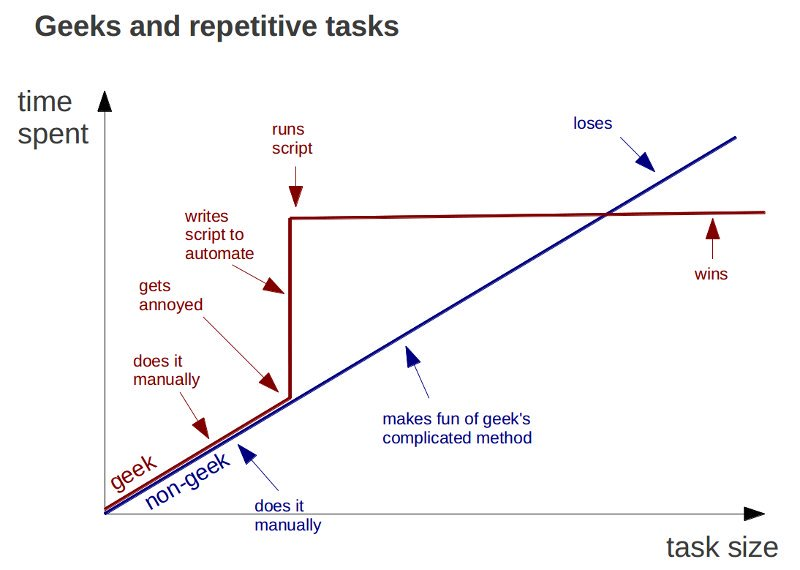
\includegraphics[height=0.8\textheight]{Geeks.jpg}

\end{frame}


%\begin{frame}[plain]
\begin{frame}
Or, adding SysAdmins into the mix:

\centering
\vspace{10pt}
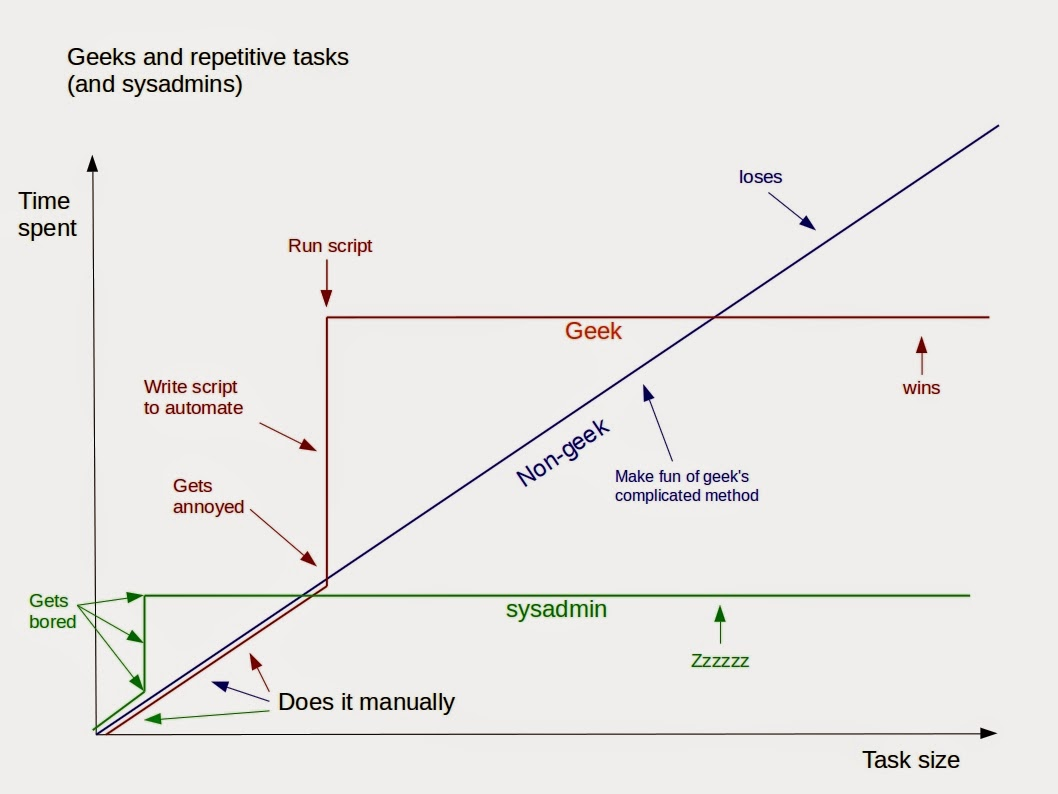
\includegraphics[height=0.8\textheight]{Geeks2.jpg}

\end{frame}


\subsection{Recommended Books}

\begin{frame}

For these Programming Tools lectures, I strongly recommend two books:

\begin{center}
	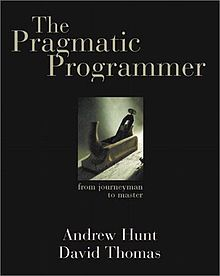
\includegraphics[width=0.27\textwidth]{tpp}
	\hspace{2cm}
	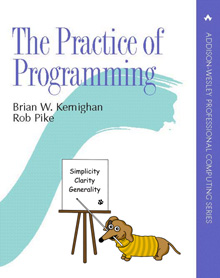
\includegraphics[width=0.27\textwidth]{tpop}
\end{center}

    \begin{itemize}
    \item
    \alert{The Pragmatic Programmer (PP)}, by \alert{Hunt \& Thomas}.
    The carpentry metaphor - and a series of excellent Programming Tips -
    comes from there.

    \pause
    \item
    \alert{The Practice of Programming (PoP)}, by \alert{Kernighan \& Pike}.
    %There's some overlap with \alert{The Pragmatic Programmer},

    \end{itemize}

    Both books are brilliant expositions of expert-level
    programming craft.
\end{frame}

\subsection{Contents}

\begin{frame}[fragile]
  Today, we'll cover:
      \begin{itemize}
        \item
          \alert{Programmer's Editors:} Use a single editor well.
        \item
	  \alert{Automating Compilation:} Use make.
        \item
   	  \alert{Multi-Directory Programs and Libraries:} How to lay out
	  programs in multiple directories, a Makefile per directory.
        \item
	  \alert{Automating Compilation:} alternatives to make.
	\end{itemize}
    \pause

    Notes:


    \begin{itemize}
    \item
    The handout (these slides) and a tarball (of examples and tools) are available on CATE and
    \verb+http://www.doc.ic.ac.uk/~dcw/c-tools-2020/lecture1/+

    \item
    As a shorthand \alert{tarball 01.intlist} refers to the directory
    called {\bf 01.intlist} inside the examples tarball.
    Each directory contains a README file (and indeed there's a top-level README).
    Read them - and if they tell you to do something, do it right away!
    \end{itemize}

\end{frame}

\section{Programmer's Editors}
\subsection{Use a Single Editor Well (PP tip 22)}

\begin{frame}
  \begin{itemize}
    \item
	  Hunt \& Thomas write (in Tip 22):
\begin{quote}
Use a Single Editor Well:
The editor should be an extension of your hand;
make sure your editor is configurable,
extensible and programmable.
\end{quote}
    \pitem
    As a programmer, you will spend \alert{years of your life} editing programs.

    \item
    Coding might be 80\% thinking and 20\% typing, but your
    typing must not interfere with your thought process.

    \pitem
    So: Explore several programmer's editors, then choose one,
    and learn to become \alert{expert in it}.

    \pitem
    That includes: learning \alert{how to plug external tools in}.

    \pitem
    Which editor?
    \pause
    It's more than my life's worth to tell you which editor to use.

    \pitem
    Why? Because programmers are notoriously sectarian when it comes to..
  \end{itemize}
\end{frame}

\begin{frame}[plain]
\setbeamercolor{col}{fg=yellow, bg=black}
%works \begin{beamercolorbox}[wd=1.0\textwidth, ht=1.0\textheight]{col}
%but even better 1.1 instead:-)
\begin{beamercolorbox}[wd=1.1\textwidth, ht=1.1\textheight]{col}
\centering
\vspace{70pt}

\includegraphics[width=0.8\textwidth]{editorWars.png}
\end{beamercolorbox}
\end{frame}

\begin{frame}
  \begin{itemize}
    \item
       The leading Programmer's editors are (probably) \alert{vim} and \alert{emacs}:


\includegraphics[width=0.3\textwidth]{vimLogo}

\includegraphics[width=0.3\textwidth]{emacsLogo}

    \pitem IDEs such as \alert{Idea} and \alert{CLion}
          provide an editor, an automated compilation system
	  and a debugging environment.
	  If you're going to use an IDE,
          learn how to use it well, and
          how to extend and program it.

     \pitem
     Note that \alert{Hunt \& Thomas} aren't much in favour of
     IDEs.  Neither am I:-)
  \end{itemize}
\end{frame}

\begin{frame}
Actually, it's well known that \alert{Real Programmers use Butterflies}
to edit source code:

\centering
\vspace{10pt}
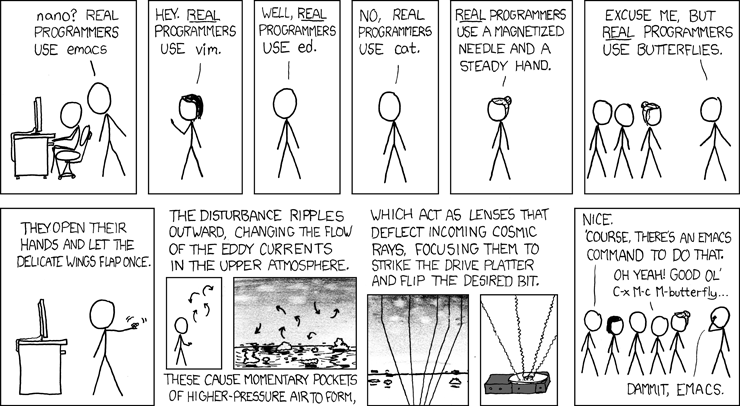
\includegraphics[height=0.8\textheight]{real_programmers.png}

\end{frame}

\section{Automatic Compilation}
\subsection{Make (tarball 01.intlist)}

\begin{frame}[fragile]
    When multi-file C programming, there are \alert{many source files}, eg:
    \par\noindent
    \begin{center}
      \includegraphics<1->[height=4cm]{diagram-0.pdf}
    \end{center}
    \par\noindent
    \pause
    \begin{itemize}
      \item Module \alert{intlist} comprising two files (interface \alert{intlist.h} and implementation \alert{intlist.c}) - defining a list-of-integers type,
      \pitem A unit test program \alert{testlist.c}, that uses and tests \alert{intlist},
      \pitem A separate basic definitions header file \alert{defns.h},
      \pitem and a main program \alert{avgwordlen.c}, that uses intlists to do something vaguely useful.
      %(reads words from a file, builds a list of the lengths of those words, and then computes the average word length).
    \end{itemize}
\end{frame}

\begin{frame}[fragile]
    \begin{itemize}
    \item
    So, what should we compile?  what should we link?
    \pitem
    What we shouldn't do: \alert{gcc -Wall *.c}.  Why not?  Try it out and see!

    \pitem
    Without Make, the correct way to make gcc compile and link everything is:

    \begin{enumerate}
    \pause
    \item
    Tell gcc to compile every .c file onto a corresponding object (.o) file:
\begin{verbatim}
  gcc -Wall -c *.c
\end{verbatim}

    \pause
    \item
    Then link each main program's .o file with the .o files of the modules it uses, creating a named executable:

\begin{verbatim}
  gcc avgwordlen.o intlist.o -o avgwordlen
  gcc testlist.o intlist.o -o testlist
\end{verbatim}

    \end{enumerate}

    \pitem
    But this is really painful, far too complex for us to do repeatedly.

    \pitem
    We \alert{need a tool to handle automatic compilation and linking for us}.

    \pitem
    That tool is \alert{make}.
    \pause
    But for it to do the job, we have to \alert{tell it the rules}:
    when should each .c file be recompiled, and when should each executable be relinked from it's
    collection of object files.

    \end{itemize}

\end{frame}

\begin{frame}[fragile]

    \begin{itemize}
    \item
    To understand more generally when files need recompiling and linking,
    \alert{dependencies} between the files are vital,
    determined by the \alert{\#include} structure.
    \pause
    See this via:
\begin{verbatim}
grep '#include' *.[ch] | grep '"'
\end{verbatim}

    \pitem
    Which gives:
{\small
\begin{verbatim}
intlist.c:#include "intlist.h"
avgwordlen.c:#include "intlist.h"
avgwordlen.c:#include "defns.h"
testlist.c:#include "intlist.h"
\end{verbatim}
}

    \pitem \alert{intlist.c} includes \alert{intlist.h}
            (to check implementation vs interface).
    \item \alert{avgwordlen.c} includes \alert{intlist.h} (because it uses intlists) and \alert{defns.h}, etc
%   \item \alert{testlist.c} includes \alert{intlist.h}

    \pitem
    {\bf Make} uses such file dependencies,
    encoded in a {\bf Makefile},
    to automatically compile and link your programs.

    \item
    The Makefile contains dependency rules between
    \alert{target} and \alert{source} files with
    \alert{optional actions} (commands) to generate each
    target from the corresponding sources.
    \end{itemize}

\end{frame}

\begin{frame}[fragile]

\begin{itemize}
\item
    Here's the Makefile for our example.  It starts with some \alert{variable} or \alert{macro}
    definitions:
\small
\begin{verbatim}
CC      = gcc
CFLAGS  = -Wall
BUILD   = testlist avgwordlen
\end{verbatim}

\verb+$(CC)+ sets which C compiler to use,
\verb+$(CFLAGS)+ is the C compiler flags, \verb+$(BUILD)+ the targets to build.
Note that environment variables automatically become macros, eg \verb+$(HOME)+
represents your home directory.

\pitem
The remainder of the Makefile lists the target/sources/action rules:

\begin{verbatim}
all:    $(BUILD)
clean:
        /bin/rm -f $(BUILD) *.o core
\end{verbatim}

\pause
\begin{verbatim}
testlist:       testlist.o intlist.o
avgwordlen:     avgwordlen.o intlist.o
avgwordlen.o:   intlist.h defns.h
testlist.o:     intlist.h
intlist.o:      intlist.h
\end{verbatim}

\end{itemize}

\end{frame}


\begin{frame}[fragile]

\begin{itemize}
      \item
	Note that Make needs very few explicit dependencies and even fewer explicit actions,
	because it already knows that \alert{intlist.o} depends on \alert{intlist.c},
	and how to compile \alert{.c} files onto the corresponding \alert{.o} file.

      \pitem
      So, when you write the rule:
\begin{verbatim}
intlist.o:      intlist.h
\end{verbatim}

      (and a \verb+intlist.c+ file exists in the current directory)

      \pause
      Make expands it to the more complete compilation rule:

\begin{verbatim}
intlist.o:         intlist.c intlist.h
        $(CC) $(CFLAGS) -c intlist.c
\end{verbatim}

      \pitem
	This rule declares that \alert{intlist.o} is up
	to date only if it is \alert{newer than intlist.c and intlist.h}.
	If \alert{intlist.o doesn't exist} or \alert{is older than either file},
	then the action is triggered - compiling \alert{intlist.c}, producing \alert{intlist.o}.
      \pitem
        \alert{make} takes optional target names on the command line
	(defaulting to the first target),
        then performs the \alert{minimum number of actions}
	needed to bring the desired targets \alert{up to date},
	based on the \alert{timestamps} of the target and source files.
	
%      \pitem
%        Common extra targets include
%	\alert{test}, alert{tar} and \alert{install},
%	as in:
%
%\small
%\begin{verbatim}
%install:        avgwordlen
%        install -m0755 avgwordlen $(HOME)/bin/$(ARCH)
%\end{verbatim}

\end{itemize}

\end{frame}

\begin{frame}[fragile]

\begin{itemize}
      \item
       For example, if \alert{intlist.h} is altered, you run \alert{make},
       that builds the target \alert{all}, which recursively applies all
       the rules checking timestamps and concludes that...

       \pitem
       ...\alert{intlist.c},
       \alert{testlist.c} and \alert{avgwordlen.c} need recompiling,
       and then the new \alert{testlist.o} and \alert{avgwordlen.o}
       need relinking against the new \alert{intlist.o}, giving the
       2 executables \alert{testlist} and \alert{avgwordlen}.

      \pitem
      If, instead, \verb+make+ is run after \alert{intlist.c} is modified,
      it figures out that it needs to recompile \alert{intlist.c},
      and relink both executables against the
      new \alert{intlist.o}.

      \pitem
      If, instead, \verb+make+ is run after nothing is modified,
      it figures out that nothing needs to be done.
      This \alert{parsimonious} property of Make is its best feature!

      \pitem
      Of course, you have to keep the dependencies in your \verb+Makefile+
      up to date, otherwise \verb+make+ may not know to recompile something.

      \pitem
      It's easy to auto-generate Makefiles for
      single directory C projects containing a single main program and
      any number of modules -
      see tarball {\bf 02.c-mfbuild} and {\bf 03.perl-mfbuild} for two
      attempts.

      \pitem 
      Make continues to work well as you add modules, unit test programs, extra standalone .h files,
      and more main programs - all in a single directory.  It never \alert{runs out of steam} because there are too many source files.
      %Summary: \alert{Always use make,} or some similar tool.
      %Keep your Makefile up to date, optionally auto-generating it.
      %Google \alert{make tutorial} for more info.


\end{itemize}

\end{frame}

\subsection{Multi-directory Projects (tarball 04.intlist-with-lib)}

\begin{frame}[fragile]
\begin{itemize}
  \item
  As a C project gets larger, you may wish to break it into several
  sub-directories.

  \pitem
  Core concept: each sub-directory contains:
  \begin{itemize}
    \item
    One or more \alert{modules} (each a paired .c and .h file as usual).
    \item
    Ideally these modules should only depend on each other, and
    the C standard library.
    \item
    Along with any associated test programs.
    \item
    Plus a Makefile that compiles all the .c files, builds all the test
    programs, and builds a \alert{library} containing the \alert{.o}
    files belonging to those modules.
  \end{itemize}

  \pitem
  Let's split our existing intlist and avgwordlen directory up.

  \item
  What to split?
  \pause
  The intlist module is:
    \begin{itemize}
    \item
    Logically separate.
    \item
    Reusable - whenever we want a list of integers.
    \item
    Depends on only the standard library.
    \end{itemize}

  \item
  That is, it's \alert{highly cohesive}.

  \item
  So: it's perfect for splitting out into a library sub-directory.

  \item
  In tarball directory \alert{04.intlist-with-lib}, you'll see
  what we have done to achieve this.

\end{itemize}
\end{frame}

\begin{frame}[fragile]
\begin{itemize}
  \item
  There's a separate \alert{lib} sub-directory, let's explore it first:
  
  \item
  \alert{lib} contains \alert{intlist.c, intlist.h, testlist.c} (all unmodified) and it's own Makefile,
  \pause
  which builds two core targets:
  \begin{itemize}
    \item
    The executable \alert{testlist}.
    \item
    The library \alert{libintlist.a} containing \alert{intlist.o}.
  \end{itemize}
  \pitem
  To do this, \alert{lib/Makefile} has the following new parts:
\begin{verbatim}
LIB     =       libintlist.a
LIBOBJS =       intlist.o
BUILD   =       testlist $(LIB)
...
$(LIB):         $(LIBOBJS)
        ar rcs $(LIB) $(LIBOBJS)
\end{verbatim}

%\pitem
%In BUILD, I've added \verb+$(LIB)+ as an extra target.

\pitem
The new rule says that \verb+$(LIB)+ depends on \verb+$(LIBOBJS)+,
i.e. \verb+libintlist.a+ depends on \verb+intlist.o+, and that the action invokes 
\alert{ar} - the tool that builds library files.

\end{itemize}
\end{frame}

\begin{frame}[fragile]
\begin{itemize}
\item
The top-level directory contains \alert{avgwordlen.c}, \alert{defns.h} and a Makefile,
\pause
containing the following new parts:
\begin{verbatim}
CFLAGS  =       -Wall -Ilib
LDLIBS  =       -Llib -lintlist
BUILD   =       libs avgwordlen
\end{verbatim}

\pitem
In CFLAGS, \verb+-Ilib+ tells the C compiler to search for include files in
the lib directory.

\pitem
In LDLIBS, \verb+-Llib+ tells the linker to search for libraries in the lib directory, and \verb+-lintlist+ tells the linker
to link the intlist library in.

\pitem
In BUILD, I've added \alert{libs} before \alert{avgwordlen}.
Later down the main Makefile, we see a rule to make \alert{libs}:
\begin{verbatim}
libs:
        cd lib; make
\end{verbatim}

\pitem
This tricks Make, with it's \alert{single directory} view of the world,
into first building everything in the lib sub-directory,
before building \alert{avgwordlen} in the current directory.

\end{itemize}
\end{frame}

\subsection{Multi-directory Projects (tarball 05.libintlist)}

\begin{frame}[fragile]
\begin{itemize}
\item
You'll also notice the \alert{clean} target now reads:
\begin{verbatim}
clean:
        /bin/rm -f $(BUILD) *.o core
        cd lib; make clean
\end{verbatim}
which makes it clean in both directories.

\pitem
In tarball \alert{05.libintlist} and \alert{06.avgwordlen-only},
you'll see how to split the intlist module out completely from the
avgwordlen application that uses intlists.

\item
In brief: \alert{05.libintlist} contains only the files from
the \alert{lib} directory.

\pitem
It's Makefile adds a new \alert{install} target to install the library into
your \verb+~/c-tools/lib/x86_64+ directory,
and install intlist.h into \verb+~/c-tools/include+.

\pitem
After running \verb+make install+ in \alert{05.libintlist}, your
\verb+~/c-tools+ library permanently contains the intlist ADT, for you to
reuse whenever you like - as shown in \alert{06.avgwordlen-only}.

\pitem
Left for you to work through!

\end{itemize}
\end{frame}

\subsection{CMake (tarball 07.intlist-with-cmake)}

\begin{frame}[fragile]

    \begin{itemize}
      \item
        I recommend learning Make thoroughly, and personally I find it's
	all I need.

      \pitem
	But if you find that keeping Makefiles up to date
        begins to bore you (especially at large scale), there are
        alternatives - or frontends - to Make:
      \pitem
	For example \alert{CMake} and Gnu \alert{autoconf} -
	both generate \alert{Makefiles} automatically from simpler
	inputs, and are supposed to scale well.
        %Let's briefly look at \alert{CMake}:

      \pitem
      In tarball \alert{07.intlist-with-cmake} you will find a copy of our
      familiar intlist-with-lib example, in which the \alert{only}
      differences are that the Makefiles have been replaced with
      CMakeLists.txt files, and the README has been modified to explain it.

      \pitem
      Go through that, and you'll get a taste of how CMake lists files
      are constructed.  But CMake is over complex and messy for my tastes.
      %Also, any tool that needs to be run in it's own \verb+build+
      %subdirectory in order to leave the source code directory uncluttered
      %is too messy for me!

      \pitem
      In a future lecture, I'll also describe an experimental tool called
      \alert{cbuild} that I've built in the last month, that tries to be a simpler
      version of cmake without all the mess.  Like cmake, it needs no rules because
      it searches every .c file for \verb+#include+ lines each time.
      %that uses
      %simple declarations in build files - it needs no rules because it searches every
      %.c file for \verb+#include+ lines every time - so works out the dependencies
      %and then executes them without using make.

    \end{itemize}

\end{frame}

\end{document}
